% mnras_template.tex
%
% LaTeX template for creating an MNRAS paper
%
% v3.0 released 14 May 2015
% (version numbers match those of mnras.cls)
%
% Copyright (C) Royal Astronomical Society 2015
% Authors:
% Keith T. Smith (Royal Astronomical Society)

% Change log
%
% v3.0 May 2015
%    Renamed to match the new package name
%    Version number matches mnras.cls
%    A few minor tweaks to wording
% v1.0 September 2013
%    Beta testing only - never publicly released
%    First version: a simple (ish) template for creating an MNRAS paper

%%%%%%%%%%%%%%%%%%%%%%%%%%%%%%%%%%%%%%%%%%%%%%%%%%
% Basic setup. Most papers should leave these options alone.
\documentclass[a4paper,fleqn,usenatbib]{mnras}

% MNRAS is set in Times font. If you don't have this installed (most LaTeX
% installations will be fine) or prefer the old Computer Modern fonts, comment
% out the following line
\usepackage{newtxtext,newtxmath}
% Depending on your LaTeX fonts installation, you might get better results with one of these:
%\usepackage{mathptmx}
%\usepackage{txfonts}

% Use vector fonts, so it zooms properly in on-screen viewing software
% Don't change these lines unless you know what you are doing
\usepackage[T1]{fontenc}
\usepackage{ae,aecompl}
\usepackage{longtable}


%%%%% AUTHORS - PLACE YOUR OWN PACKAGES HERE %%%%%

% Only include extra packages if you really need them. Common packages are:
\usepackage{graphicx}	% Including figure files
\usepackage{amsmath}	% Advanced maths commands
\usepackage{amssymb}	% Extra maths symbols
\usepackage{xspace}
\usepackage{hyperref}



% added by DH
\newcommand{\numax}{\mbox{$\nu_{\rm max}$}\xspace}
\newcommand{\Dnu}{\mbox{$\Delta \nu$}\xspace}
\newcommand{\dnu}{\mbox{$\delta \nu$}\xspace}
\newcommand{\muHz}{\mbox{$\mu$Hz}\xspace}
\newcommand{\teff}{\mbox{$T_{\rm eff}$}\xspace}
\newcommand{\logg}{\mbox{$\log g$}\xspace}
\newcommand{\feh}{\mbox{$\rm{[Fe/H]}$}\xspace}
\newcommand{\msun}{\mbox{$\mathrm{M}_{\sun}$}\xspace}
\newcommand{\rsun}{\mbox{$\mathrm{R}_{\sun}$}\xspace}
\newcommand{\kepler}{\emph{Kepler}\xspace}
\newcommand{\hipparcos}{\emph{Hipparcos}\xspace}
\newcommand{\gaia}{\emph{Gaia}\xspace}



%%%%%%%%%%%%%%%%%%%%%%%%%%%%%%%%%%%%%%%%%%%%%%%%%%

%%%%% AUTHORS - PLACE YOUR OWN COMMANDS HERE %%%%%

% Please keep new commands to a minimum, and use \newcommand not \def to avoid
% overwriting existing commands. Example:
%\newcommand{\pcm}{\,cm$^{-2}$}	% per cm-squared

%%%%%%%%%%%%%%%%%%%%%%%%%%%%%%%%%%%%%%%%%%%%%%%%%%

%%%%%%%%%%%%%%%%%%% TITLE PAGE %%%%%%%%%%%%%%%%%%%

\title[The Kepler Smear Campaign]{The \kepler Smear Campaign I: An Asteroseismic Catalogue of Bright Red Giants}

% This author list is not final! If you think you should be in a different position please do not hesitate to say so.
\author[B. J. S. Pope et al.]{Benjamin J. S. Pope,$^{1,2,3}$\thanks{E-mail: benjamin.pope@nyu.edu}
Guy R. Davies,$^{4,5}$
Keith Hawkins,$^{6,7}$
Timothy R. White,$^{5,8}$\newauthor
Daniel Huber,$^{9,10,11}$
Ashley Chontos,$^{9}$
Victor Silva Aguirre,$^{5}$
Victoria Antoci,$^{5}$\newauthor
Suzanne Aigrain,$^{3}$ 
Timothy R. Bedding,$^{10,5}$
Jie Yu,$^{10,5}$ 
Amalie Stokholm,$^{5}$\newauthor
Timothy van Reeth,$^{5,10}$
David W. Latham,$^{12}$,
Allyson Bieryla,$^{12}$
Gilbert A. Esquerdo,$^{12}$\newauthor
and friends
\\
% List of institutions
$^{1}$Center for Cosmology and Particle Physics, Department of Physics, New York University, 726 Broadway, New York, NY 10003, USA\\
$^{2}$NASA Sagan Fellow\\
$^{3}$Oxford Astrophysics, Denys Wilkinson Building, University of Oxford, OX1 3RH, Oxford, UK\\
$^{4}$School of Physics and Astronomy, University of Birmingham, Birmingham B15 2TT, UK\\
$^{5}$Stellar Astrophysics Centre, Department of Physics and Astronomy, Aarhus University, Ny Munkegade 120, DK-8000 Aarhus C, Denmark\\
$^{6}$Department of Astronomy, The University of Texas at Austin, 2515 Speedway Boulevard, Austin, TX 78712, USA\\
$^{7}$Department of Astronomy, Columbia University, 550 W 120th St, New York, NY 10027, USA\\
$^{8}$Research School of Astronomy and Astrophysics, Mount Stromlo Observatory, The Australian National University, Canberra, ACT 2611, Australia\\
$^{9}$Institute for Astronomy, University of Hawai‘i, 2680 Woodlawn Drive, Honolulu, HI 96822, USA\\
$^{10}$Sydney Institute for Astronomy (SIfA), School of Physics, University of Sydney, NSW 2006, Australia\\
$^{11}$SETI Institute, 189 Bernardo Avenue, Mountain View, CA 94043, USA\\
$^{12}$Harvard-Smithsonian Center for Astrophysics, 60 Garden Street, Cambridge, MA 02138, USA
}

% These dates will be filled out by the publisher
\date{Accepted XXX. Received YYY; in original form ZZZ}

\pubyear{2018}

% Don't change these lines
\begin{document}
\label{firstpage}
\pagerange{\pageref{firstpage}--\pageref{lastpage}}
\maketitle

% Abstract of the paper
\begin{abstract}
Here we present the first data release of the \kepler Smear Campaign, using collateral `smear' data obtained by \kepler to reconstruct light curves of 102~stars too bright to have been otherwise targeted. We describe the pipeline developed to extract and calibrate these light curves, and show that we attain photometric precision comparable to stars analyzed by the standard pipeline in the nominal \kepler mission. In this Paper, we focus in particular on a subset of these consisting of 64~red giants for which we detect solar-like oscillations. Using high-resolution spectroscopy from the Tillinghast Reflector \'{E}chelle Spectrograph (TRES) together with asteroseismic modelling, we obtain the stellar densities and derive masses, radii and ages of~34 of these red giant and red clump stars as benchmarks. All source code, light curves, TRES spectra, and asteroseismic and stellar parameters are publicly available as a \kepler legacy sample.
\end{abstract}

% Select between one and six entries from the list of approved keywords.
% Don't make up new ones.
\begin{keywords}
asteroseismology -- techniques: photometric -- stars: variable: general
\end{keywords}

%%%%%%%%%%%%%%%%%%%%%%%%%%%%%%%%%%%%%%%%%%%%%%%%%%

%%%%%%%%%%%%%%%%% BODY OF PAPER %%%%%%%%%%%%%%%%%%

\section{Introduction}
\label{intro}

% The \kepler Space Telescope, operated by NASA, was launched in 2009 to obtain photometry of hundreds of thousands of stars in a field in Cygnus-Lyra, in order to detect a statistically-useful sample of transiting exoplanets \citep{2010Sci...327..977B}. It achieved this primary goal, showing that exoplanets are common around Sun-like stars \citep{2013ApJ...766...81F,2013PNAS..11019273P,2014ApJ...795...64F}, though with the failure of two reaction wheels, the mission was cut short and there remain substantial uncertainties on these estimates. \kepler was revived as a two-wheeled mission, K2, with its third axis balanced against solar radiation pressure. K2 is therefore constrained to point in the ecliptic plane, which it surveys in a succession of $\sim 80$~day Campaigns. In this paper, we will deal exclusively with data from the nominal \kepler mission before this change.

% Beyond searching for planets, 
\kepler has revolutionized the field of asteroseismology for solar-like oscillations \citep{2010PASP..122..131G}. It has yielded the first detection of gravity-mode period spacings in a red giant \citep{rggmodes}, enabling probes of interior rotation of red giants \citep{rggmoderotation} and distinguishing between hydrogen- and helium-burning cores \citep{rggmodehelium}. It has also permitted the determination of ages and fundamental parameters of main-sequence stars as cool as the Sun and hotter \citep{silvaages}, including planet-hosting stars \citep{huberplanetages,silvaplanetages,2018MNRAS.479.4786V}, revealing the most ancient known planetary system, dating back to the earliest stages of the galaxy \citep{ancientplanets}. By comparing asteroseismic stellar ages to stellar rotation periods, \citet{angusgyro} have shown that gyrochronology models cannot fit the data with a single relation, leading \citet{vansadersgyro} to suggest a qualitative change in dynamo mechanism as stars age through the main sequence. 

A major outcome of the \kepler asteroseismology programme is a legacy sample of extremely well characterized stars that can serve as benchmarks for future work \citep{keplerlegacy1,keplerlegacy2}. In conjunction with spectroscopy, \citet{hawkinsapogee} have been able to produce a large sample of stars with precise elemental abundances by fitting spectroscopic data with \logg and \teff fixed to asteroseismically-determined values. It is necessary to calibrate such a study against benchmark stars with very precisely-determined parameters, which in practice requires nearby bright stars that are amenable to very high signal-to-noise spectroscopy plus asteroseismology \citep{creeveybenchmark}, parallaxes \citep{hawkinsbenchmarks}, and/or interferometry \citep{casagrandebenchmark,creeveybenchmark2}. This is especially important in the context of the \gaia mission \citep{gaia}, which has recently put out its second data release of 1,692,919,135 sources, including 1,331,909,727 with parallaxes \citep{gaiadr2}. These data will form the basis of many large surveys and it is vital that they are calibrated correctly. To this end, 34~FGK stars including both giants and dwarfs have been chosen as \gaia-ESO benchmark stars for which metallicities \citep{gaiabenchmark1}, effective temperatures and asteroseismic surface gravities \citep{gaiabenchmark3}, and relative abundances of $\alpha$ and iron-peak elements \citep{gaiabenchmark4} have been determined. This includes only four main sequence stars much cooler than the Sun, due to the paucity of such stars with asteroseismology. This has been accompanied by the release of high resolution spectra \citep{gaiabenchmark2} and formed the basis of extensions to lower metallicities \citep{gaiabenchmark5}, stellar twin studies \citep{gaiabenchmarktwins} and comparisons of stellar abundance determination pipelines \citep{gaiabenchmarkabundances}. Furthermore, by combining asteroseismology with optical interferometry, it has been possible to determine fundamental parameters of main-sequence and giant stars with unprecedented precision \citep{huber12,thetacygwhite,white15}. 

Brighter \kepler stars are therefore ideal benchmark targets, since photometry can be most easily complemented by \gaia parallaxes, interferometric diameters, and high resolution spectroscopy.  
Unfortunately, the \kepler field was deliberately placed to minimize overall the number of extremely bright stars on the detectors, so that only a dozen stars brighter than~6th~magnitude landed on silicon \citep{2010ApJ...713L..79K}. This was because stars brighter than $Kp \sim 11$ saturate the CCD detectors, with their flux distributed along a bleed column and rendering those pixels otherwise unusable. Furthermore, due to the limited availablility of bandwidth to download data from the spacecraft, only a fraction \textcolor{red}{What fraction?} of pixels on the \kepler detectors are actually downloaded. The result of these two target selection constraints is that photometry was obtained for only \textcolor{red}{a small number} of saturated stars in the \kepler field, while many bright targets were ignored. In the K2 mission \citep{k2early}, very saturated stars have been observed with `halo photometry' using unsaturated pixels in a specially-determined region around bright stars, including the Pleiades \citep{halo}, Aldebaran \citep{aldebaran}, and $\rho$~Leonis \citep{rholeo}. Unfortunately, in the legacy \kepler sample, photometry of such saturated stars was rarely attempted.

\citet{orig_smear} noted a way to obtain photometry of every target on-silicon in \kepler using a data channel normally used for calibration, even if active pixels were not allocated and downloaded. \kepler employs an inter-line transfer CCD as its detector, which successively shuffles each row of pixels down to the edges of the chip to be read out. Because the \kepler camera lacks a shutter, the detector is exposed to light during the readout process, with the result that fluxes in each pixel are contaminated by light collected from objects in the same column. This is a particularly serious issue for faint objects in the same detector column as brighter stars, and it is important to calibrate this at each readout stage. Six rows of blank `masked' pixels were allocated in each column to measure the smear bias; furthermore, six `virtual' rows were recorded at the end of the readout, with the result that twelve rows of pixels sample the smear bias in each column. \citet{orig_smear} realized that these encode the light curves of bright targets in a 1D projection of the star field. The masked and virtual smear registers each receive $\sim 1/1034$ of the incident flux in each column. If this is dominated by the light from a single star, the flux combining both smear registers is equivalent to that of a star $\sim 6.8$~times fainter. 

In \citet{smear}, we demonstrated a method for extracting precise light curves of bright stars in \kepler and K2, and presented light curves of a small number of variable stars as examples to illustrate this method. In this paper we present smear light curves of all unobserved or significantly under-observed stars brighter than $Kp=9$ in the \kepler field. This sample mostly consists of red giants and hot stars, containing only a few FG dwarfs. We find no transiting planets, but detect \textcolor{red}{$M$}~new eclipsing binaries, and measure solar-like oscillations in 34~red giants. We do not model hot stars or FG dwarfs in great detail, but provide some discussion and initial classification of interesting variability. For eclipsing binaries, we present the results of light-curve modelling to precisely determine their parameters. For the oscillating red giants that constitute the bulk of the sample, we determine the asteroseismic parameters \numax and \Dnu, and therefore stellar masses and \logg measurements; and we and obtain high-resolution spectroscopy with the Tillinghast Reflector \'{E}chelle Spectrograph (TRES), from whose spectra we derive stellar parameters and elemental abundances constrained by asteroseismic parameters. These asteroseismic constraints can be compared to those from \gaia, offering the opportunity both to test asteroseismic scaling relations and combine both datasets to refine the benchmark star properties further.

We have made all new data products and software discussed in this paper publicly available, and encourage interested readers to use these in their own research.   

\section{Method}
\label{method}

We have obtained smear light curves for our sample of red giant stars with the \texttt{keplersmear} pipeline as described in Section~\ref{photometry}, performed asteroseismology on all of these to extract \numax and therefore \logg as described in Section~\ref{asteroseismology}, and combined these with TRES spectra to obtain chemical abundances as described in Section~\ref{spectroscopy}. 

\subsection{Sample}
\label{sample}

We selected as our sample all stars on-silicon in \kepler with $Kp<9$ that were targeted for fewer than an arbitrary $8$ quarters, including those stars that were entirely unobserved. A number of these lay at the edge of a detector, with the result that in some cadences the centroid of the star did not lie on the chip; light curves from these targets were found to be of extremely low quality and all of these objects were discarded. After applying these criteria we obtained a list of 102 targets, which are listed in Table~\ref{all_stars} in order of their \kepler magnitude $Kp$ together with their spectral type from SIMBAD, \gaia~DR2 source identifiers, apparent~$G$ magnitudes and distances from \citet{gaiadists}, the quarters for which the stars were observed, and whether spectroscopy is available in Section~\ref{spectroscopy} and Table~\ref{stellar_props}. The \kepler spacecraft rotates between quarters, so that it cycles through four orientation `seasons' each rotated from the last by $90^{\circ}$. Some stars did not land on silicon for all seasons: we have only one season of HD~179394; two for HD~187277, HD~226754, V554~Lyr, and BD+47~2891; and three for BD+43~3064. \textcolor{red}{Aside from the restriction on stars falling on the edge of a chip}, the addition of our sample to the conventionally-observed stars makes the \kepler survey magnitude-complete down to $Kp=9$. 

In Figure~\ref{hrdiagram} we show these stars on a colour-magnitude diagram in \gaia $Bp-Rp$ and absolute~$G$ magnitudes using \gaia~DR2 calibrated distances from \citet{gaiadists}, overlaid on the \kepler sample from the Bedell \url{gaia-kepler.fun} crossmatch. The smear targets in this diagram appear to have not merely higher apparent brightnesses than the general \kepler population, but also higher intrinsic luminosities. While this could simply arise from being selected for their apparent brightness, it is worth considering whether this is because of a bias in their parallax measurements. While \gaia parallaxes for very bright stars can be subject to systematic error, we have compared these to those found by \emph{Hipparcos} \citep{vanleeuwen07b}, and found close agreement for the brightest stars, with a scatter that increases with magnitude. We therefore suggest that parallax bias is not the reason for the smear sample sitting above the remainder of the \kepler sample.

We identify the evolutionary state of objects in the main sequence versus evolved stars first from the \gaia colour-magnitude diagram in Figure~\ref{hrdiagram}. Taking a cutoff in \gaia $Bp-Rp > 1$, we identify 64 of these objects as clearly evolved systems, and the remaining~38 lie apparently on the main sequence. 

One of the main sequence objects, BD+43~3068 is a G0 dwarf with a $G$ magnitude of 8.267944 and a distance of $53.8 \pm 0.1$~pc, and it is therefore surprising that it was not included in the nominal \kepler survey as a Solar analogue: it is possible that it was previously misidentified as a giant. Regrettably, it is only possible to reconstruct a light curve with the 30~minute long cadence and therefore it is not possible to do asteroseismology on this bright, nearby solar-like star. This light curve shows neither rotational modulation (as determined by its featureless autocorrelation) nor evidence of transits.

Considering objects lying photometrically on the main sequence, from the \kepler power spectrum we identify solar-like oscillations in HD~182354 and HD~176209 at frequencies consistent with them being subgiants. \textcolor{red}{Get frequencies}.


\subsection{Photometry}
\label{photometry}

In preparing light curves of the \kepler smear stars, we follow the methods described in \citet{smear}, with some improvements. We select using RA and Dec values from the \kepler Input Catalog (KIC) \citep{kic}, and query MAST to find the corresponding mean pixel position for a given \kepler quarter. We measure the centroid of smear columns in the vicinity, and use these values to do raw aperture photometry. We find that the cosine-bell aperture used for raw photometry in \citet{smear} can in some light curves introduce position-dependent systematics and jumps. We instead in this work apply a super-Gaussian aperture, $A \propto \exp{\dfrac{-(x-x_0)}{w} ^ 4}$, where $x_0$ is the centroid and $w$ a width in pixels. The very flat top of this function helps avoid significant variation with position, while still smoothly rolling off at the edges to avoid discontinuous artefacts. We calculate this on a grid of $10\,\times$ subsampled points in pixel space so that the sharply varying edge changes column weights smoothly as a function of centroid. We extract photometry using apertures with a range of widths $w \in\{1.5,~2,~3,~4,~5\}$ pixels.

From this raw photometry we subtract a background light curve, which corrects for time-varying global systematics. Whereas in \citet{smear} we then subtract a background estimate chosen manually, for this larger set of light curves, we now choose the lowest $25\%$ of pixels by median flux as being unlikely to be contaminated by stars, and take our background level to be the median of this at each time sample. To denoise this, we fit a Gaussian Process with a 30-day timescale squared exponential kernel using \textsc{george} \citep{hodlr}, and our final background light curve is taken to be the posterior mean of this GP. 

The dominant source of residual systematic errors in nominal \kepler time series is a common-mode variation primarily due to thermal changes on board the spacecraft, an issue which is traditionally dealt with by identifying and fitting a linear combination of systematic modes \citep{pdc0,pdc1,pdc2,petigura}. We adopt the same approach here, using the \kepler Pre-search Data Conditioning (PDC) Cotrending Basis Vectors (CBVs) available from MAST, finding least-squares fits of  either the first~4 or~8 CBVs to each light curve. We note that this can subtract astrophysical signals on long timescales, such that we use and recommend 4~CBV light curves for stars with variability on timescales longer than $\sim 5$ days, but otherwise use the 8~CBV light curves. There is some room for improvement here by simultaneously modelling astrophysical and instrumental variations, but this is beyond the scope of this paper. In the following, we will use the light curves with the lowest 6.5~hr Combined Differential Photometric Precision (CDPP) \citep{cdpp} out of all apertures, as calculated with the \textsc{k2sc} implementation \citep{k2sc}. This is not necessarily the optimal choice for all red giants, especially those with oscillations on a 6.5~h timescale, but is a reasonable proxy nevertheless for white noise and leads to satisfactory results upon visual inspection of the present sample.


\begin{figure*}
\noindent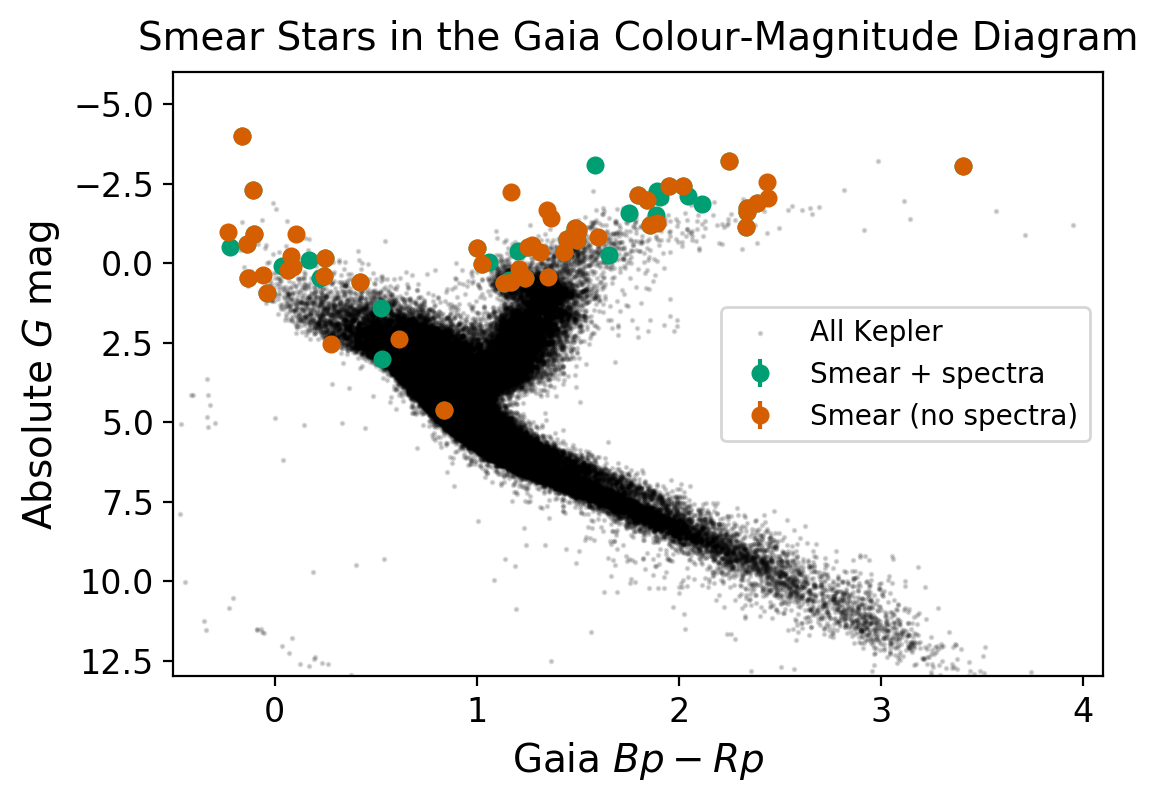
\includegraphics[width=15cm,keepaspectratio]{gaia_kepler_hr.png}

\caption{\label{hrdiagram}
\gaia colour-magnitude diagram of the Smear Campaign stars (orange and teal) overlaid on the sample of \kepler stars with \gaia parallax $\text{SNR} > 25$ (black), using the Bedell \url{gaia-kepler.fun} crossmatch and \gaia~DR2 calibrated distances from \citet{gaiadists}. The smear sample includes giants and hot main-sequence stars. Those giants for which TRES spectroscopy have been obtained are highlighted in teal. An interactive version of this diagram is available as supplementary material from the journal or at \url{benjaminpope.github.io/data/cmd_smear.html}.}
\end{figure*}

Because the smear data are collected along an entire CCD~column, there is the risk of contamination from sufficiently bright sources. This is especially true in doing asteroseismology of red giants, where the low-amplitude stochastically-excited oscillations can be washed out in a power spectrum by the coherent high amplitude variations of a classical pulsator, even if the background star is much fainter. We can assess the importance of this contamination by considering the differences between odd and even quarters: because the \kepler spacecraft rotates $90^{\circ}$ between successive quarters, any contaminant will lie in the same column as a smear target only every second quarter, falling in the other quarters in the same row but not necessarily the same column. We have therefore generated Lomb-Scargle periodograms \citep{lomb,scargle} of each light curve, clipped for outliers, and considering only odd and even quarters, and visually inspected these for significant differences. In the great majority of cases they closely resemble one another, indicating that contamination is at worst a minor effect. In the case of HD~181878, a red giant, there is clear and significant contamination from a $\delta$~Scuti variable, as is seen in Figure~\ref{contamination}. 


\begin{figure}
\noindent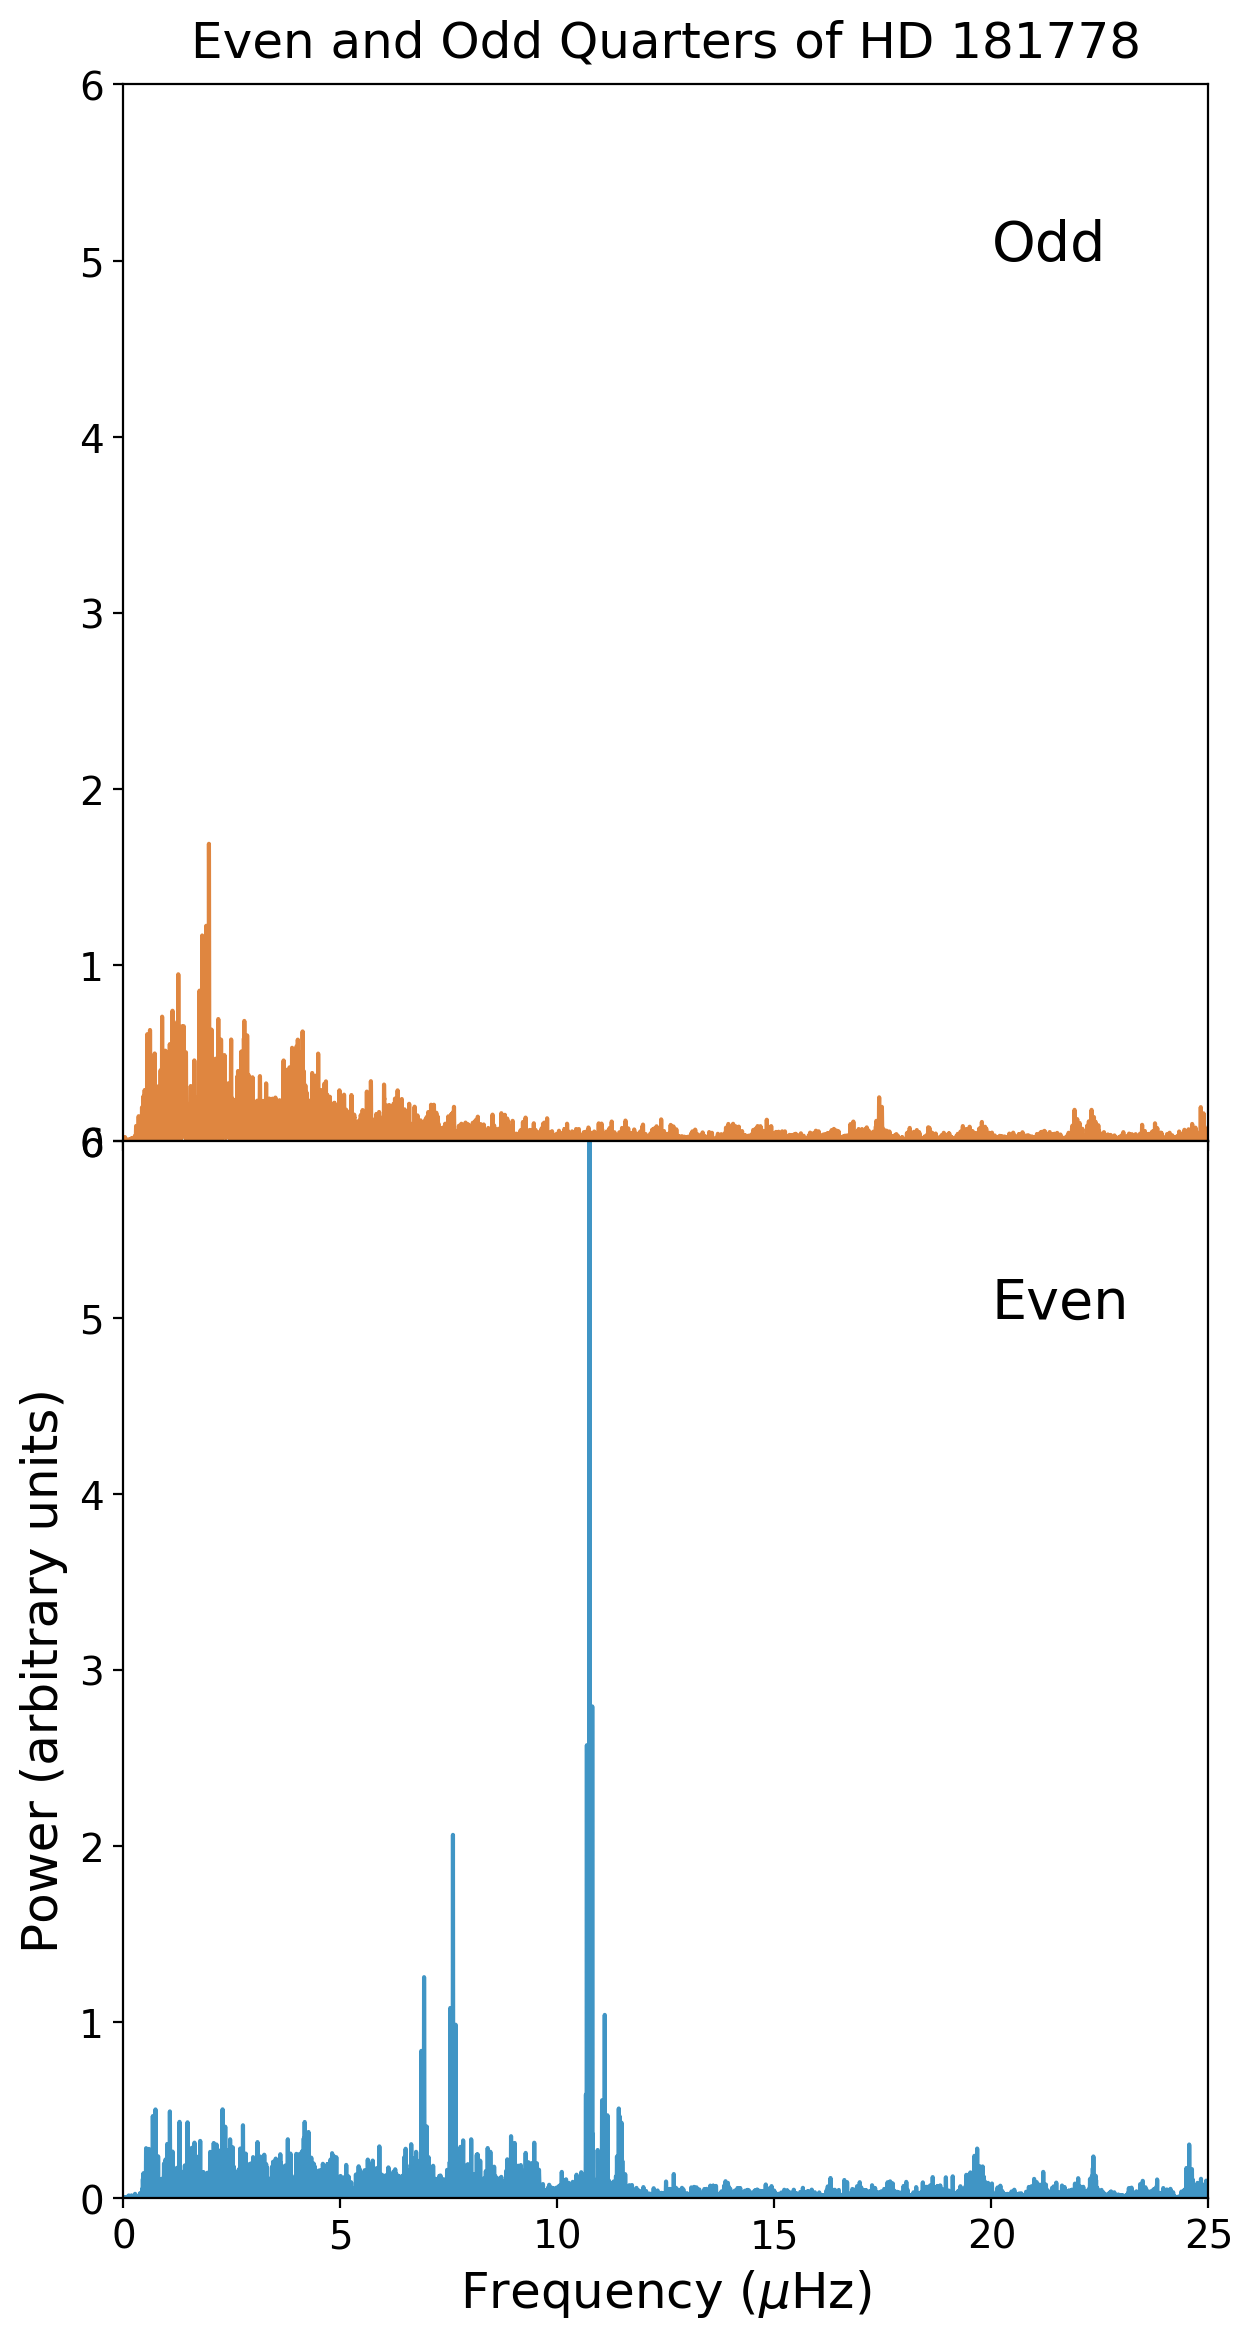
\includegraphics[width=8cm,keepaspectratio]{contam_HD_181778.png}

\caption{\label{contamination}
Power spectra of odd and even quarters of HD~181778. It is clear from inspection that while odd quarters have the power spectrum expected of a giant star, even quarters have very high amplitude coherent oscillations typical of a $\delta$~Scuti variable.}
\end{figure}


\begin{table*}
\caption{The full set of underobserved and unobserved stars for which new light curves have been produced in this smear catalogue.         Calibrated \gaia distances are from \citet{gaiadists}.         Some objects, such as HD~185351, were observed in long cadence in some quarters and short cadence in others, and this is noted accordingly.         The eclipsing binary V2083~Cyg was detected by \gaia, but a parallax could not be obtained in DR2, possibly due to binary motion.        Variability classes are determined by inspection, having their usual abbreviations.         EV denotes an ellipsoidal variable, but some of these could be rotation and spot modulation.        $\gamma\,\text{Dor} /\delta\,\text{Sct}$ denotes a $\gamma\,\text{Dor} /\delta\,\text{Sct}$ hybrid, not uncertainty.        H+S denotes a `hump and spike' star.        Question marks indicate uncertainty, and dashes -- that no significant variability is observed.\label{all_stars}\label{all_stars}}
\begin{tabular}{ccccccccc}
\hline \hline
Object & KIC & Spectral Type & $Kp$ & $G$ & $Bp-Rp$ & \gaia Distance & TRES & Variability \\
 &  & (SIMBAD) & (mag) & (mag) & (mag) & (pc) &  & Class \\
\hline
14 Cyg & 7292420 & G8.5IIIbFe-0.5 & 5.490 & 4.882 & 1.091 & $41.2^{+0.1}_{-0.1}$ & -- & EV \\
BD+36 3564 & 1575741 & F5II-III & 8.128 & 4.923 & 0.529 & $50.6^{+0.4}_{-0.4}$ & \checkmark & RG \\
BD+39 3577 & 4989821 & G8III & 8.131 & 5.152 & 1.171 & $81.5^{+0.6}_{-0.6}$ & \checkmark & RG \\
BD+39 3882 & 4850372 & A2V & 8.259 & 5.279 & 0.107 & $172.6^{+3.3}_{-3.2}$ & -- & Irregular \\
BD+42 3150 & 7091342 & B9III & 8.350 & 5.370 & -0.055 & $194.3^{+7.0}_{-6.6}$ & -- & ? \\
BD+42 3367 & 7447756 & B5V & 7.271 & 5.410 & -0.106 & $347.3^{+13.0}_{-12.1}$ & \checkmark & LPV \\
BD+42 3393 & 6870455 & M1III & 7.664 & 5.313 & 2.047 & $306.4^{+10.3}_{-9.6}$ & \checkmark & LPV \\
BD+43 3064 & 8075287 & G7IIIa & 8.284 & 5.598 & 1.061 & $133.1^{+0.7}_{-0.7}$ & \checkmark & RG \\
BD+43 3068 & 8006792 & B1.1III+B2.5/3V: & 8.308 & 5.632 & -0.062 & $1044.7^{+116.6}_{-95.6}$ & -- & -- \\
BD+43 3171 & 7810954 & M3III & 8.373 & 5.176 & 2.250 & $475.2^{+35.1}_{-30.7}$ & \checkmark & LPV \\
BD+43 3213 & 7747499 & A5III & 8.311 & 5.881 & 0.246 & $125.2^{+6.2}_{-5.7}$ & \checkmark & LPV \\
BD+47 2825 & 10337574 & B2III & 8.251 & 5.864 & -0.276 & $1000.6^{+82.6}_{-71.1}$ & -- & EB \\
BD+47 2891 & 10347606 & K1III & 8.680 & 5.985 & 1.283 & $135.8^{+0.3}_{-0.3}$ & -- & RG \\
BD+48 2904 & 11085556 & K5 & 8.487 & 6.055 & 1.645 & $263.5^{+3.9}_{-3.8}$ & -- & RG \\
BD+48 2955 & 10988024 & K2 & 7.961 & 6.091 & 1.584 & $683.8^{+12.4}_{-11.9}$ & \checkmark & RG \\
HD 174177 & 9630812 & M4-IIIa & 6.575 & 5.228 & 2.725 & $288.9^{+13.1}_{-12.0}$ & -- & $\gamma\,\text{Dor}$ \\
HD 174676 & 7420037 & K0 & 7.481 & 6.144 & 1.448 & $238.9^{+1.5}_{-1.4}$ & \checkmark & LPV \\
HD 174829 & 7339102 & K1III & 6.967 & 6.264 & 1.237 & $144.2^{+0.6}_{-0.6}$ & \checkmark & RG \\
HD 175132 & 6020867 & K0 & 6.362 & 6.258 & 1.168 & $499.2^{+7.2}_{-7.0}$ & -- & EV \\
HD 175466 & 7340766 & B3V & 6.165 & 6.160 & -0.217 & $345.1^{+5.6}_{-5.4}$ & -- & LPV \\
HD 175841 & 4989900 & B9IIIpSi & 6.885 & 6.242 & -0.063 & $333.3^{+5.9}_{-5.7}$ & -- & $\gamma\,\text{Dor} /\delta\,\text{Sct}$ \\
HD 175884 & 6584587 & B0.5IIIn & 6.210 & 6.243 & -0.160 & $1114.0^{+70.9}_{-63.0}$ & \checkmark & RG \\
HD 176209 & 9327530 & B3Ve & 7.437 & 6.208 & -0.041 & $571.1^{+18.2}_{-17.2}$ & -- & ? \\
HD 176582 & 4136285 & K0 & 6.510 & 6.345 & 1.273 & $243.2^{+1.8}_{-1.8}$ & -- & EV \\
HD 176626 & 7943968 & G8II & 6.933 & 6.395 & 1.176 & $160.7^{+0.8}_{-0.8}$ & -- & EV \\
HD 176894 & 6267965 & M0II-III & 7.700 & 6.171 & 2.031 & $409.4^{+3.8}_{-3.7}$ & -- & $\gamma\,\text{Dor}$ \\
HD 177697 & 4994443 & K5 & 7.300 & 6.248 & 1.892 & $317.7^{+2.7}_{-2.7}$ & -- & RG \\
HD 177781 & 2970780 & B5V & 7.744 & 6.383 & -0.232 & $298.6^{+3.9}_{-3.8}$ & -- & $\gamma\,\text{Dor} /\delta\,\text{Sct}$ \\
HD 178090 & 6675338 & A2IV & 6.758 & 6.483 & 0.119 & $223.9^{+1.7}_{-1.6}$ & -- & LPV \\
HD 178797 & 10064283 & K0 & 7.312 & 6.532 & 1.486 & $295.8^{+2.5}_{-2.5}$ & \checkmark & RG \\
HD 178910 & 11288450 & G5 & 7.864 & 6.587 & 1.003 & $259.5^{+1.8}_{-1.8}$ & \checkmark & RG \\
HD 179394 & 7105221 & K5 & 7.575 & 6.600 & 1.754 & $433.1^{+4.2}_{-4.1}$ & \checkmark & -- \\
HD 179395 & 6593264 & A0V & 7.168 & 6.658 & -0.003 & $139.6^{+1.1}_{-1.1}$ & -- & EV \\
HD 179396 & 3838362 & K5 & 8.001 & 6.549 & 1.892 & $583.0^{+8.5}_{-8.3}$ & \checkmark & RG \\
HD 179959 & 10265370 & K4III & 6.280 & 6.696 & 1.798 & $585.0^{+9.1}_{-8.9}$ & \checkmark & RG \\
HD 180312 & 4551179 & A2 & 7.970 & 6.797 & 0.172 & $241.0^{+2.1}_{-2.1}$ & \checkmark & RG \\
HD 180475 & 11656042 & A3 & 7.664 & 6.810 & 0.351 & -- & \checkmark & RG \\
HD 180658 & 6195870 & A2 & 7.932 & 6.840 & 0.225 & $188.8^{+6.4}_{-6.0}$ & \checkmark & RG \\
HD 180682 & 5177450 & K5 & 6.617 & 6.530 & 2.116 & $476.9^{+5.9}_{-5.8}$ & \checkmark & LPV \\
HD 181022 & 3946721 & A2V & 6.496 & 6.841 & 0.035 & $224.8^{+1.8}_{-1.7}$ & \checkmark & LPV \\
HD 181069 & 4049174 & A0 & 6.279 & 6.852 & 0.059 & $217.8^{+3.4}_{-3.3}$ & \checkmark & RG \\
HD 181097 & 4149233 & A5 & 7.920 & 6.855 & 0.421 & $180.0^{+1.0}_{-1.0}$ & \checkmark & RG \\
HD 181328 & 12456737 & A3 & 7.182 & 6.862 & 0.252 & $254.5^{+4.1}_{-4.0}$ & \checkmark & LPV \\
HD 181521 & 5180075 & K0 & 6.939 & 6.928 & 1.391 & $355.0^{+3.5}_{-3.4}$ & -- & $\gamma\,\text{Dor} /\delta\,\text{Sct}$ \\
HD 181596 & 11910615 & M3 & 7.050 & 5.403 & 3.406 & $494.7^{+34.9}_{-30.6}$ & \checkmark & RG \\
HD 181597 & 11555267 & K5III & 6.040 & 6.863 & 1.841 & $591.1^{+8.1}_{-7.8}$ & \checkmark & RG \\
HD 181681 & 5092997 & B9 & 6.864 & 7.070 & 0.067 & $233.9^{+1.7}_{-1.7}$ & \checkmark & RG \\
HD 181778 & 7816792 & B8V & 7.545 & 7.034 & -0.221 & $321.5^{+3.7}_{-3.6}$ & \checkmark & RG \\
HD 181878 & 4830109 & M1 & 6.698 & 6.614 & 2.334 & $353.9^{+3.3}_{-3.3}$ & \checkmark & RG \\
HD 181880 & 3337423 & M5 & 7.982 & 6.719 & 2.337 & $492.9^{+5.5}_{-5.4}$ & \checkmark & RG \\
HD 182354 & 2156801 & B9 & 6.320 & 7.143 & -0.055 & $226.5^{+2.4}_{-2.3}$ & -- & RG \\
HD 182531 & 11188366 & B9IV & 7.955 & 7.145 & -0.037 & $175.5^{+2.6}_{-2.5}$ & \checkmark & RG \\
\hline
\end{tabular}
\end{table*}

\input{all_Stars2.tex}

\subsection{Asteroseismology}
\label{asteroseismology}

While~64 red giants have been identified in this sample, for some of these, by visual inspection it is clear that the timescale of their variability is of the same order as a \kepler quarter and they are thus badly affected by systematics and systematics correction. From the 34 giants for which there is high-SNR shorter-timescale variability, we have attempted to extract the asteroseismic parameters \numax and $\langle \Dnu \rangle$ \citep{KB95,2013ARA&A..51..353C}. These constrain fundamental stellar parameters as through these scaling relations: 

\begin{equation}
\label{scaling}
\numax \propto \dfrac{g}{g_{\sun}} \cdot \left(\dfrac{\teff}{\teff_{\sun}}\right)^{\dfrac{1}{2}}
\end{equation}

and

\begin{equation}
\langle \Dnu \rangle \propto \sqrt{\langle \rho \rangle} = \sqrt{\dfrac{M}{\msun} \left(\dfrac{R}{\rsun}\right)^{-3}}
\end{equation}

We follow the method of \citet{2016AN....337..774D}, obtaining a Lomb-Scargle periodogram of the smoothed time series according to the method of \citet{2011MNRAS.414L...6G}. We then conduct a Markov Chain Monte Carlo fit to this, applying the combined granulation and oscillation model of \citet{2014A&A...570A..41K}, consisting of two Harvey profiles for the granulation \citep{1985ESASP.235..199H}, a Gaussian envelope for the stellar oscillations, and a white noise background for instrumental noise. We find that the marginal posterior distribution for the Gaussian envelope is well-approximated by a single Gaussian, and take its median and standard deviation to be our estimates for \numax and its uncertainty.

To estimate \Dnu, we divide the power spectrum through by the granulation and noise models to obtain a signal-to-noise spectrum, and fit a sum of Lorentzians separated by mean large (\Dnu) and small (\dnu) separations to the part of this spectrum in the vicinity of \numax. In practice, for this dataset, \dnu is poorly constrained, but mean $\langle \Dnu \rangle$ is typically well-constrained and its posterior marginal distribution is well-represented by a single Gaussian as with \numax. 

We obtain good estimates of these asteroseismic parameters for 35 targets, presented in Table~\ref{astero_table}. In many of the remainder of cases, we find that the very-low-frequency ($\lesssim 2\muHz$) oscillations are affected by filter artefacts from detrending, and we are not able to obtain good estimates for these stars. 

Once \numax has been estimated, we use the asteroseismic scaling relation for \numax \citep[Equation~\ref{scaling};][]{KB95} to estimate \logg in order to inform extraction of chemical abundances from spectra. Using the initial spectroscopic estimate of \teff, which is not significantly informed by \numax, we propagate uncertainties in \numax with Monte Carlo sampling. 

For eight stars, we find that the asteroseismic fit is unsatisfactory: for BD+39~388 we cannot detect the expected oscillations; for BD+43~3064 there are significant peaks but these are not consistent with the pattern expected from a red giant; for HD~179959 and HD~187217 we suspect contamination with the oscillations of a second giant, which is hard to remove from smear light curves; while for HD~188629, HD~188639 and HD~188875 we can extract a \numax but not a robust \Dnu. One star in our sample, the retired~A star HD~185351, has a mode envelope that is not well fit by our model. The smear light curve for this star has already been published by \citet{2017MNRAS.464.3713H}, who showed with detailed asteroseismic modelling that it had a zero-age main sequence mass of $\sim 1.60 \msun$ and used it to calibrate the convective overshoot parameter for low-luminosity red giants. The bulk asteroseismic modelling presented here should therefore be considered to be superseded by the more detailed model of \citet{2017MNRAS.464.3713H}. 

\begin{table}
\caption{Bulk asteroseismic parameters \Dnu, \numax, and $\epsilon$ for the red giant sample as discussed in Section~\ref{asteroseismology}.\label{astero_table}\label{stellar_props}}
\begin{tabular}{cccc}
\hline \hline
Object & \Dnu & \numax & $\epsilon$ \\
 & (\muHz) & (\muHz) &  \\
\hline
BD+36 3564 & $0.95 \pm 0.03$ & $5.08 \pm 0.10$ & $0.83 \pm 0.20$ \\
BD+39 3577 & $1.68 \pm 0.01$ & $13.27 \pm 0.32$ & $0.74 \pm 0.06$ \\
BD+42 3150 & $4.22 \pm 0.03$ & $38.32 \pm 0.96$ & $0.70 \pm 0.07$ \\
BD+43 3171 & $0.42 \pm 0.05$ & $1.98 \pm 0.05$ & $0.80 \pm 0.17$ \\
BD+43 3213 & $0.49 \pm 0.01$ & $2.56 \pm 0.06$ & $1.01 \pm 0.07$ \\
BD+48 2904 & $2.85 \pm 0.01$ & $23.13 \pm 0.72$ & $0.86 \pm 0.08$ \\
BD+48 2955 & $0.90 \pm 0.01$ & $5.44 \pm 0.08$ & $0.81 \pm 0.05$ \\
HD 174020 & $0.56 \pm 0.02$ & $2.48 \pm 0.10$ & $0.89 \pm 0.08$ \\
HD 174829 & $1.28 \pm 0.01$ & $7.95 \pm 0.16$ & $0.78 \pm 0.06$ \\
HD 175740 & $5.93 \pm 0.01$ & $64.33 \pm 0.78$ & $1.00 \pm 0.02$ \\
HD 175884 & $1.12 \pm 0.01$ & $7.07 \pm 0.11$ & $0.96 \pm 0.08$ \\
HD 176209 & $4.22 \pm 0.08$ & $36.08 \pm 0.77$ & $0.87 \pm 0.06$ \\
HD 178797 & $1.03 \pm 0.02$ & $6.34 \pm 0.09$ & $0.74 \pm 0.29$ \\
HD 178910 & $3.64 \pm 0.02$ & $32.06 \pm 0.31$ & $0.83 \pm 0.05$ \\
HD 179396 & $3.76 \pm 0.02$ & $31.02 \pm 0.44$ & $0.92 \pm 0.03$ \\
HD 180312 & $4.17 \pm 0.02$ & $33.84 \pm 0.28$ & $0.96 \pm 0.04$ \\
HD 180475 & $0.82 \pm 0.00$ & $4.34 \pm 0.10$ & $0.68 \pm 0.03$ \\
HD 180658 & $4.00 \pm 0.02$ & $33.76 \pm 0.50$ & $0.90 \pm 0.05$ \\
HD 180682 & $0.77 \pm 0.05$ & $3.68 \pm 0.08$ & $1.07 \pm 0.15$ \\
HD 181022 & $0.38 \pm 0.01$ & $1.58 \pm 0.03$ & $0.70 \pm 0.10$ \\
HD 181069 & $4.43 \pm 0.01$ & $41.46 \pm 0.32$ & $0.90 \pm 0.02$ \\
HD 181097 & $1.61 \pm 0.02$ & $11.16 \pm 0.14$ & $0.72 \pm 0.36$ \\
HD 181597 & $3.11 \pm 0.01$ & $25.84 \pm 0.25$ & $0.97 \pm 0.02$ \\
HD 181778 & $2.56 \pm 0.02$ & $22.86 \pm 0.29$ & $0.72 \pm 0.06$ \\
HD 181880 & $1.04 \pm 0.01$ & $6.54 \pm 0.10$ & $0.76 \pm 0.05$ \\
HD 182354 & $2.66 \pm 0.01$ & $24.73 \pm 0.37$ & $0.74 \pm 0.04$ \\
HD 182531 & $1.03 \pm 0.00$ & $6.47 \pm 0.09$ & $0.86 \pm 0.03$ \\
HD 182692 & $4.66 \pm 0.01$ & $44.38 \pm 0.47$ & $0.87 \pm 0.02$ \\
HD 182694 & $5.71 \pm 0.01$ & $69.78 \pm 1.02$ & $0.94 \pm 0.25$ \\
HD 183124 & $4.39 \pm 0.01$ & $39.59 \pm 0.29$ & $0.95 \pm 0.03$ \\
HD 185286 & $0.72 \pm 0.01$ & $4.23 \pm 0.10$ & $0.73 \pm 0.08$ \\
HD 188537 & $1.55 \pm 0.01$ & $13.40 \pm 0.34$ & $0.72 \pm 0.07$ \\
HD 189750 & $4.16 \pm 0.04$ & $36.14 \pm 0.58$ & $0.94 \pm 0.08$ \\
HD 226754 & $1.19 \pm 0.01$ & $7.41 \pm 0.19$ & $0.74 \pm 0.08$ \\
\hline
\end{tabular}
\end{table}


\subsection{Spectroscopy}
\label{spectroscopy}

For the whole red giant sample, we have obtained high-resolution spectroscopy with TRES in order to constrain stellar parameters and elemental abundances. Operating with spectral resolving power $R=44 000$, we obtain signal-to-noise ratios of tens to hundreds per resolution element. We note that this resolution and SNR are sufficient for an exploratory study, but for more detailed analysis it will be desirable to use APOGEE or similar instruments to obtain greater spectral coverage. From this observing run we have~34 unique targets with seismic \logg and spectra, one more star than the \gaia-ESO benchmark set and a significant addition to the ensemble of bright red giants with asteroseismic parameter determinations. These are unfortunately not the same~34 unique targets as for the asteroseismic analysis presented above in Section~\ref{asteroseismology}: due to observing constraints, we were unable to obtain spectra for BD+42~3150, BD+48~2904, HD~176209, HD~182354, HD~189636AB, or HD~189750.

To derive stellar parameters from our TRES spectra, we initially run the Stellar Parameter Classification \citep[SPC:][]{spc} code to determine \teff and \logg, using the SPC \teff to inform the asteroseismic estimation of \logg from \numax. For deriving abundances, \teff is fixed from the results of an initial SPC fit, while \logg is fixed to the seismic values. The other stellar atmospheric parameters including the microturbulent velocity ($v_{\text{mic}}$), and broadening (convolution by $V_{\text{mac}}$, $v_{\sin{i}}$ and the instrumental line profile) as well as [Fe/H] and chemical abundances for 20 chemical species are derived using the Brussels Automatic Code for Characterizing High accUracy Spectra \citep[BACCHUS:][]{bacchus}, and the results from this calculation are displayed in Table~\ref{stellar_props}. BACCHUS uses an interpolation scheme through a grid of MARCS model atmospheres \citep{Gustafsson2008} in combination with TURBOSPECTRUM \citep{Alvarez1998, Plez2012}. For the calculation of synthetic spectra, atomic line information has been taken from the fifth version of the Gaia-ESO linelist (Heiter et al., in preparation). Additionally we used the molecular species for CH \citep{Masseron2014}, CN, NH, OH, MgH  C$_{2}$ (T. Masseron, private communication). The SiH molecular information is adopted from the Kurucz linelists and the information for TiO, ZrO, FeH, CaH from B. Plez (private communication). 

Individual elemental abundances are derived by first fixing the stellar atmospheric parameters to those determined above. Spectra are then synthesized  in regions centered around an absorption  feature of the element we want to derive. The spectra generated will have different [X/Fe] values. A $\chi^2$ minimization procedure is then done to derive the best fitting abundance for each line. The reported abundances are the median [X/Fe] value of the various line regions for a given element. { \bf Ben: Maybe remove this if we do not actually implement line-by-line differential; Do we have a TRES Arcturus spectrum.} Abundance uncertainties reported are the standard error in the line-by-line abundance ratios. Where only one line exists for a given element, we conservatively assume the standard error is 0.10~dex. In principle, these uncertainties are underestimated because there they do not include the errors driven by imperfect stellar parameter values and other systematic errors arising, for instance, from incorrect line list data. We do note, however, thus use of asteroseismology really reduces the uncertainties caused by the stellar parameters \citep[see][for a longer discussion on this]{hawkinsapogee}. To achieve the most precise abundances we have derived them using  both with and without a line-by-line differential approach with respect to Arcturus ($\alpha$~Bo\"{o}tis) using the method described by \citet{gaiabenchmark4} and the Arcturus abundances from \citep{hawkinsapogee}. The results of these absolute abundance calculations {\bf without the line-by-line differential analysis implemented?}, are presented in Tables~\ref{elems1},~\ref{elems2} and~\ref{elems3}. Because for most elements Arcturus differential abundances are not available, these are provided as supplementary online-only material. No abundances for oxygen could be reliably derived for any of the stars in our spectroscopic sample by either method.

\begin{table*}
\caption{Fundamental stellar parameters for the red giant sample as determined jointly by asteroseismology (asteroseismic \logg; Section~\ref{asteroseismology}) and spectroscopy (RV, \teff, \logg, [M/H], $V\sin{i}$, and SNR; Section~\ref{spectroscopy}.)\label{stellar_props}\label{stellar_props}}
\begin{tabular}{ccccccc}
\hline \hline
Object & RV & \teff & \logg & [M/H] & $V\sin{i}$ & SNR \\
 & (km/s) & (K) &  &  & (km/s) &  \\
\hline
BD+36 3564 & $-77.84 \pm 0.05$ & $4100 \pm 50$ & $1.57 \pm 0.01$ & $-0.63 \pm 0.08$ & $5.54 \pm 0.50$ & 71.8 \\
BD+39 3577 & $-14.81 \pm 0.07$ & $4737 \pm 50$ & $2.02 \pm 0.01$ & $-0.41 \pm 0.08$ & $4.78 \pm 0.50$ & 92.8 \\
BD+43 3171 & $-16.32 \pm 0.11$ & $3656 \pm 50$ & $1.14 \pm 0.01$ & $-1.20 \pm 0.08$ & $4.54 \pm 0.50$ & 68.9 \\
BD+43 3213 & $-14.16 \pm 0.16$ & $3901 \pm 50$ & $1.26 \pm 0.01$ & $-0.16 \pm 0.08$ & $6.82 \pm 0.50$ & 57.3 \\
BD+48 2955 & $1.66 \pm 0.04$ & $4143 \pm 50$ & $1.60 \pm 0.01$ & $-0.60 \pm 0.08$ & $5.33 \pm 0.50$ & 31.7 \\
HD 174020 & $-14.84 \pm 0.08$ & $3781 \pm 50$ & $1.24 \pm 0.02$ & $-1.03 \pm 0.08$ & $5.38 \pm 0.50$ & 120.1 \\
HD 174829 & $10.15 \pm 0.03$ & $4381 \pm 50$ & $1.78 \pm 0.01$ & $-0.48 \pm 0.08$ & $4.71 \pm 0.50$ & 112.2 \\
HD 175740 & $-8.81 \pm 0.04$ & $4875 \pm 50$ & $2.71 \pm 0.01$ & $-0.12 \pm 0.08$ & $3.90 \pm 0.50$ & 169.3 \\
HD 175884 & $-34.39 \pm 0.07$ & $4306 \pm 50$ & $1.72 \pm 0.01$ & $-0.41 \pm 0.08$ & $4.91 \pm 0.50$ & 144.4 \\
HD 178797 & $6.35 \pm 0.05$ & $4201 \pm 50$ & $1.67 \pm 0.01$ & $-0.63 \pm 0.08$ & $4.82 \pm 0.50$ & 77.1 \\
HD 178910 & $-14.28 \pm 0.05$ & $4560 \pm 50$ & $2.39 \pm 0.00$ & $0.12 \pm 0.08$ & $4.38 \pm 0.50$ & 76.9 \\
HD 179396 & $24.80 \pm 0.04$ & $4731 \pm 50$ & $2.39 \pm 0.01$ & $-0.24 \pm 0.08$ & $4.32 \pm 0.50$ & 82.7 \\
HD 180312 & $-21.94 \pm 0.05$ & $4868 \pm 50$ & $2.43 \pm 0.00$ & $-0.49 \pm 0.08$ & $4.25 \pm 0.50$ & 73.5 \\
HD 180475 & $-45.90 \pm 0.08$ & $4129 \pm 50$ & $1.50 \pm 0.01$ & $-0.85 \pm 0.08$ & $5.34 \pm 0.50$ & 58.4 \\
HD 180658 & $2.97 \pm 0.06$ & $4717 \pm 50$ & $2.42 \pm 0.01$ & $-0.17 \pm 0.08$ & $3.99 \pm 0.50$ & 72.3 \\
HD 180682 & $30.99 \pm 0.07$ & $4077 \pm 50$ & $1.43 \pm 0.01$ & $-1.03 \pm 0.08$ & $5.75 \pm 0.50$ & 80.1 \\
HD 181022 & $-80.39 \pm 0.16$ & $3557 \pm 50$ & $1.03 \pm 0.01$ & $-1.63 \pm 0.08$ & $4.68 \pm 0.50$ & 108.8 \\
HD 181069 & $9.99 \pm 0.05$ & $4740 \pm 50$ & $2.51 \pm 0.00$ & $-0.09 \pm 0.08$ & $3.95 \pm 0.50$ & 90.0 \\
HD 181097 & $-5.60 \pm 0.08$ & $4389 \pm 50$ & $1.93 \pm 0.01$ & $-0.39 \pm 0.08$ & $4.50 \pm 0.50$ & 69.7 \\
HD 181597 & $-13.06 \pm 0.04$ & $4612 \pm 50$ & $2.30 \pm 0.00$ & $-0.35 \pm 0.08$ & $3.51 \pm 0.50$ & 161.8 \\
HD 181778 & $-22.04 \pm 0.06$ & $4608 \pm 50$ & $2.25 \pm 0.01$ & $-0.21 \pm 0.08$ & $4.36 \pm 0.50$ & 87.6 \\
HD 181880 & $0.56 \pm 0.08$ & $4200 \pm 50$ & $1.68 \pm 0.01$ & $-0.56 \pm 0.08$ & $4.91 \pm 0.50$ & 71.2 \\
HD 182531 & $-7.34 \pm 0.05$ & $4204 \pm 50$ & $1.68 \pm 0.01$ & $-0.49 \pm 0.08$ & $4.94 \pm 0.50$ & 71.4 \\
HD 182692 & $-8.01 \pm 0.04$ & $4762 \pm 50$ & $2.54 \pm 0.00$ & $0.03 \pm 0.08$ & $4.55 \pm 0.50$ & 72.8 \\
HD 182694 & $-0.87 \pm 0.06$ & $5089 \pm 50$ & $2.75 \pm 0.01$ & $-0.19 \pm 0.08$ & $5.30 \pm 0.50$ & 187.2 \\
HD 183124 & $14.96 \pm 0.02$ & $4781 \pm 50$ & $2.49 \pm 0.00$ & $-0.27 \pm 0.08$ & $5.51 \pm 0.50$ & 114.3 \\
HD 185286 & $-13.70 \pm 0.08$ & $4090 \pm 50$ & $1.49 \pm 0.01$ & $-0.37 \pm 0.08$ & $5.98 \pm 0.50$ & 135.6 \\
HD 188537 & $-18.03 \pm 0.15$ & $4776 \pm 50$ & $2.02 \pm 0.01$ & $-0.24 \pm 0.08$ & $10.98 \pm 0.50$ & 67.0 \\
HD 226754 & $18.66 \pm 0.10$ & $4184 \pm 50$ & $1.74 \pm 0.01$ & $-0.12 \pm 0.08$ & $5.33 \pm 0.50$ & 62.5 \\
\hline
\end{tabular}
\end{table*}


\input{abundances_1.tex}
\input{abundances_2.tex}
\input{abundances_3.tex}

\section{Results}
\label{targets}

\subsection{Red Giants}
\label{rgs}

\subsubsection{Chemical Composition}
\label{chemical}
The chemical compositions for each star were measured in the $\alpha$ (Mg, Ti, Si, Ca), odd-Z (Al, Na, Cu, Sc, V), Fe-peak (Fe, Ni, Zn, Co, Cr, Mn), and neutron capture (Sr, Y, Zr, Ba, La, Nd, Eu) elemental families. This was done to asses the Galactic populations from which these stars are drawn from. The first thing to note is that the metallicity, which are tabulated in Table~\ref{stellar_props}, are to high (with $-0.51<$~[M/H]~$<$ +0.14~dex) to be considered drawn from the Galactic halo, whose peak metallicity is around --1.20 \cite[e.g.][]{Chiba2000}. Furthermore, the distance distribution, noted in Table~\ref{all_stars}, indicates that all stars are located within a few~kpc of the Sun and thus are not apart of the Galactic bulge. These alone allow us to predict that theses stars are drawn from only the Galactic thick and thin disks. We provide a detailed chemical abundance analysis below to support this claim.\\
{\bf $\alpha$ elements:}\\
\begin{figure*}
\noindent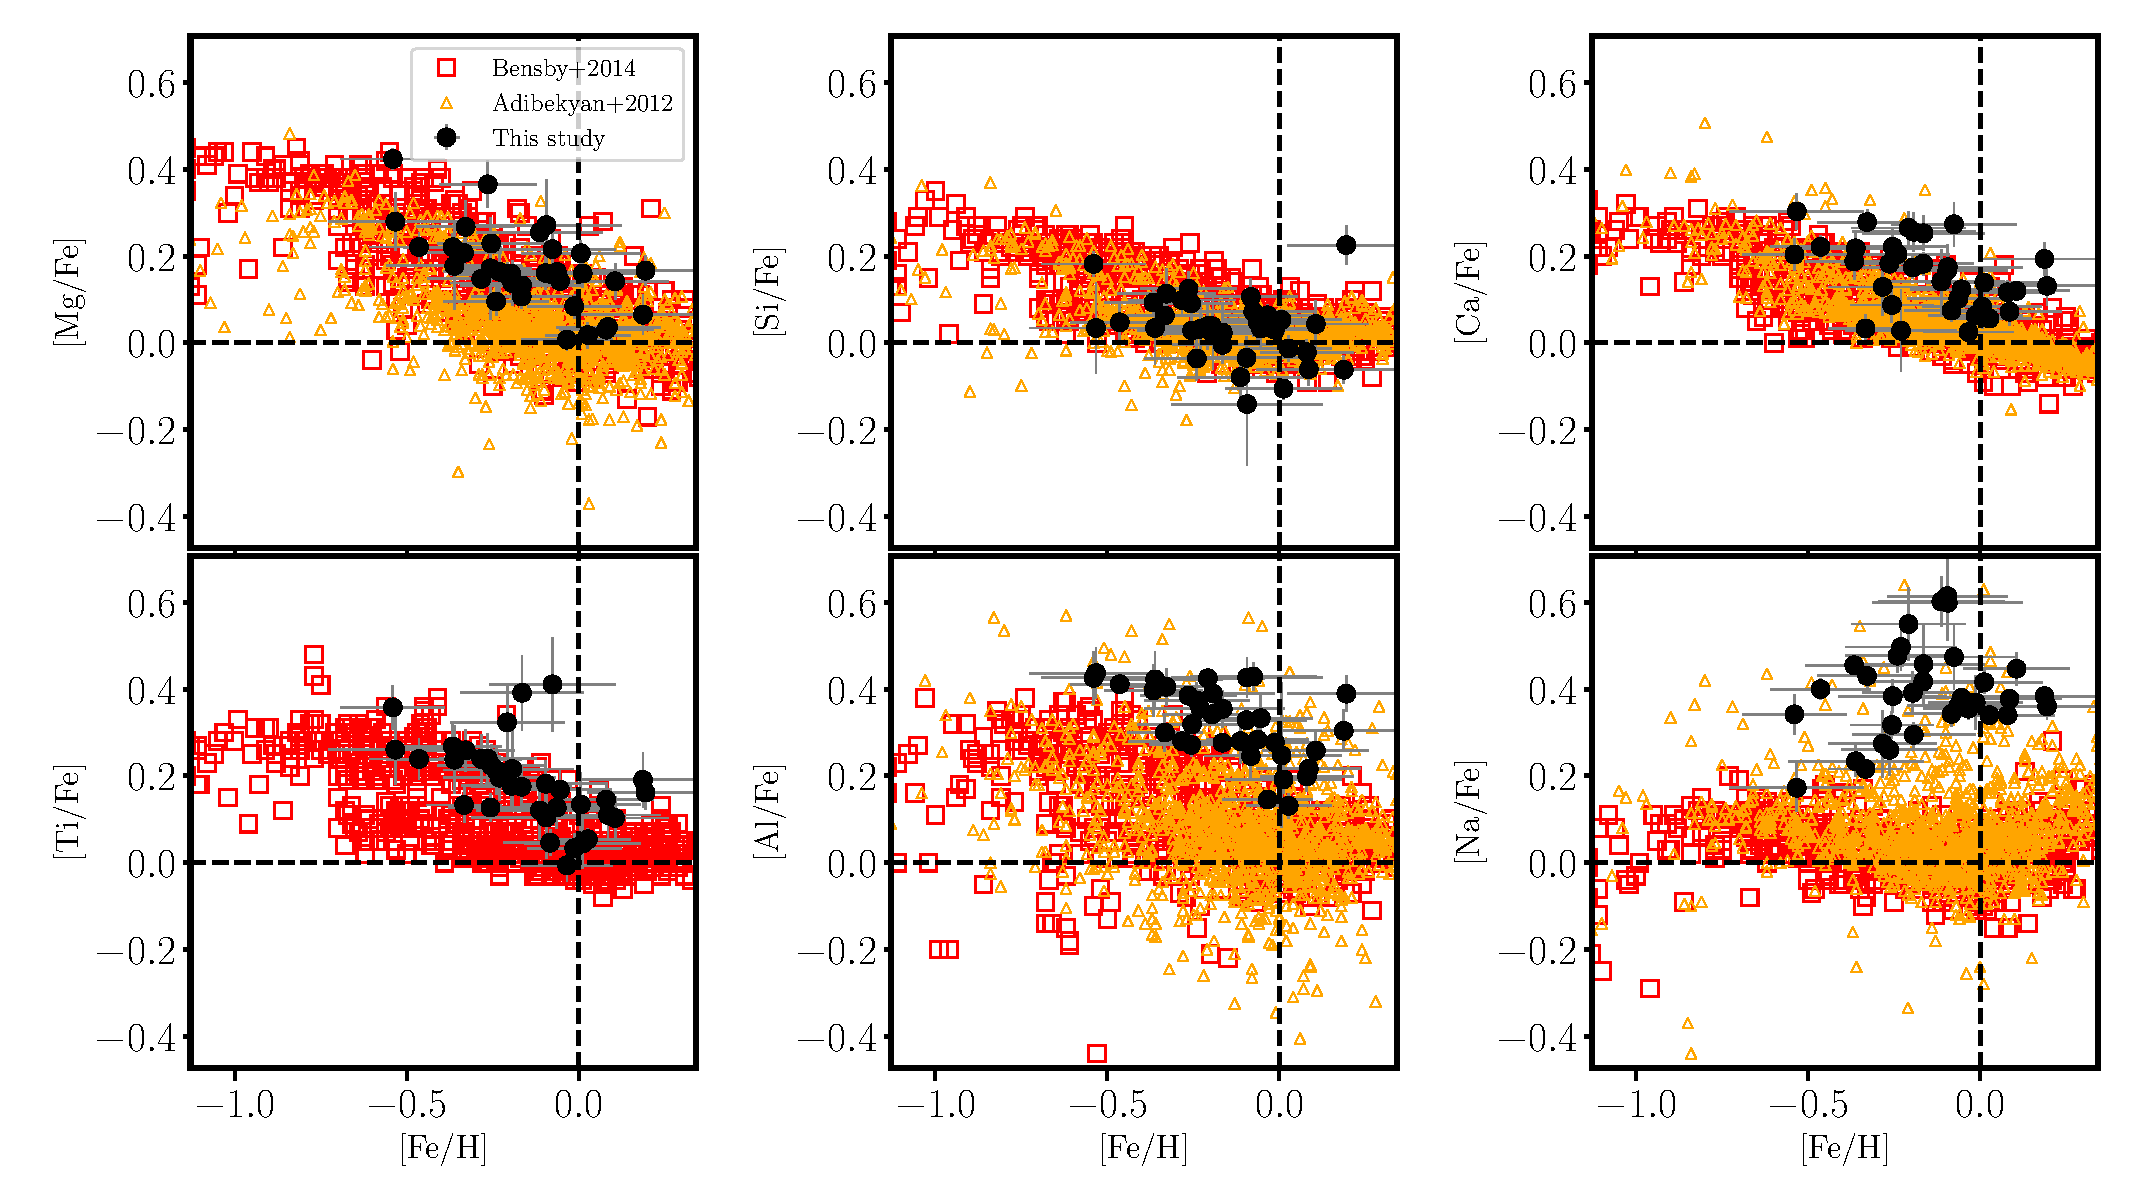
\includegraphics[width=\textwidth,keepaspectratio]{Pope_spectra_alphaele.pdf}

\caption{\label{alphael}
The [Mg/Fe], [Si/Fe], [Ca/Fe], and [Ti/Fe], [Al/Fe], [Na/Fe] abundance ratios as a function of iron on the top and bottom rows, respectively for our stars (black cirlces). We also illustrate a representative sample of Galactic disk stars from \citet[open red square,][]{Bensby2014} and \citet[open orange triangles,][]{Adibekyan2012}. } 
\end{figure*}
The $\alpha$ elements are thought to form in  variety ways during internal fusion within a star while it evolves over its life. These elements are then largely dispersed into the interstellar medium through Type~II supernovae (SNII) \citep{Matteucci2001}. The most important of these diagrams are those including the abundances of the $\alpha$ elements as a function of metallicity. It has been shown by many studies \citep[e.g.][and references therein]{Edvardsson1993, Adibekyan2012, Feltzing2013, Bensby2014}, that the Galactic thick disk and thin disk separate in the $\alpha$ elements, where the thick disk is enhanced in [Mg, Si, Ca, Ti/Fe] compared to the Galactic thin disk at a given metallicity. In Fig.~\ref{alphael}, we display the [Mg, Si, Ca, Ti/Fe] abundance ratios as a function of [Fe/H] for our stars (black circles) compared\footnote{We note that there are likely systematics between our [X/Fe] abundance scale and those of our comparison samples. We do not have the relevant data, which include several stars in common with these studies but observed with the TRES spectrograph, to asses the level of systematics.}  to representative disk stars from \cite[open red square,][]{Bensby2014} and \cite[open orange triangles,][]{Adibekyan2012}. 

For most of the stars in our sample, the [Mg, Ti, Ca/Fe] abundance ratios are enhanced. The commonly used [$\alpha$/Fe] abundance ratio is the average of Mg, Ti, Si, Ca (thus it is ([Mg/Fe] + [Ca/Fe] + [Si/Fe] + [Ti/Fe] / 4.0) ) is also enhanced in most stars. This is consistent with most stars belonging to the Galactic thick disk. Though there are a handful of stars where the typical [$\alpha$/Fe] ratio is solar. 
\\ 
{\bf Odd-Z elements:}\\
The odd-Z elements Na and Al are also shown in  Fig.~\ref{alphael}. These elements are significantly enhanced 
\\
{\bf Fe-peak elements:}\\
XX
\\ 
{\bf Neutron capture elements:}\\
XX



%place [X/Fe] vs [Fe/H] diagrams here and discuss which Galactic populations these stars come from. May also want to discuss how these span the typical Galactic populations and can act as benchmark stars for APOGEE or other large surveys 

Two of the stars in our sample also appear in the Hypatia catalogue of stellar abundances \citep{hypatia}: HD~185351 and HD~175740. The abundances reported here for HD~185351 are consistent within the large errorbars of both surveys with those reported in Hypatia, while for HD~175740 they are not. \textcolor{red}{Keith - what's going on here? Check this?}

\subsubsection{Red Clump Stars}
\label{clumpstars}

Red clump stars, which burn helium in their cores, differ significantly in their core structure from stars on the hydrogen shell burning red giant sequence. They can therefore be distinguished from hydrogen-shell burning giants asteroseismologically, due to their much higher \emph{g}-mode period spacings \citep{rggmodehelium}. 
The moniker `red clump' arises from the fact that such stars can have a very narrow range of luminosities, so that they appear as a clump in the HR diagram \citep{2016ARA&A..54...95G}. This property makes them useful standard candles to which distances can be accurately computed from photometry. Red clump stars have been used to calibrate the \gaia survey's parallaxes at long distances \citep{2017A&A...598L...4D,2017MNRAS.471..722H,2018A&A...609A.116R}. \gaia~DR2 parallaxes have a zero-point offset of $\sim 0.03$~mas \citep{gaiadr2parallax}, and in particular hierarchical models of the ensemble of \gaia clump stars can be used to accurately estimate this and thereby improve the accuracy of \gaia distances greater than a few~kpc (Hawkins et al., in prep.).

From visual inspection of the power spectra, HD~181069, HD~183124, HD~182354, HD~182692, and HD~180658 are seen to be red clump stars. A power spectrum of the best example of these, HD~183124, together with an \'{e}chelle diagram used to estimate its \emph{g}-mode period spacing, is shown in Figure~\ref{HD_183124}. While precise characterization of these stars to the necessary degree is beyond the scope of this paper, they are ideal candidates for anchoring models of the mass and metallicity dependence of red clump properties for calibrating \gaia and other distance measures. 

\begin{figure*}
\noindent\includegraphics[width=19cm,keepaspectratio]{HD_183124.png}

\caption{\label{HD_183124}
Power spectrum (left) and \'{e}chelle diagram (right) of the solar-like oscillations of the red clump star HD~183124. The modes in the power spectrum used for the \'{e}chelle diagram are highlighted with blue dots. In the \'{e}chelle diagram we see the characteristic pattern of `bumped' modes from avoided crossings between the comb of \emph{p}-modes and \emph{g}-mode oscillations with a period spacing of $\Delta \Pi = 300.1~\text{s}$.}
\end{figure*}

\subsection{Main Sequence Stars}
\label{mainseq}

For all the main sequence stars in our sample, we visually inspected light curves and power spectra to determine their variability class. In the following subsections, we will briefly comment on some of the findings. As main sequence variables are so diverse, and suited to varied science cases, we have attempted only a very preliminary study of these stars in this paper, leaving detailed analysis to future work.

\subsubsection{Classical Pulsators}
\label{pulsators}
The sample contains many $\delta\,\text{Sct}$ and $\gamma\,\text{Dor}$ variables, and several hybrid pulsators. \textcolor{red}{Simon - add text here.}
Including hotter stars, we also detect SPB pulsations in \textcolor{red}{some stars - Conny/Tim van Reeth?}. 

\subsubsection{Hump and Spike Stars}
\label{hs}

Two stars in the sample show the `hump-and-spike' morphology in their power spectra (a broad `hump' of low-amplitude oscillations dominated by one high amplitude coherent oscillation): HD~186155 (HR~7495), and HD~183362 (HR~7403), respectively the third brightest and $37^{\text{th}}$-brightest stars on silicon and the brightest two stars that show this effect. \citet{2018MNRAS.474.2774S} have recently claimed the hump-and-spike power spectra as evidence for Rossby modes. The F5 star HD~186155, identified by SIMBAD as having a giant spectral type of F5II-III, is shown by its \gaia distance to in fact lie on the main sequence. The other example is the B3e star HD~183362 at $G = -2.576$. A detailed study of these stars will be presented by Antoci et al., in prep.

Another star with a hump-and-spike spectrum is Boyajian's~Star, which shows deep enigmatic dips in brightness \citep{2016MNRAS.457.3988B}, and has faded both throughout the \kepler mission \citep{2016ApJ...830L..39M} and in relation to Harvard photographic plates from 1890 onwards \citep{2016ApJ...822L..34S}. The dimming, which is chromatic in the manner expected of heterogeneous clouds of circumstellar dust in the line of sight \citep{2018ApJ...853..130D,2018arXiv180608842B}, has been ascribed to various causes \citep[reviewed in][]{2018RNAAS...2a..16W}, most notably a cloud of exocomets surrounding the star \citep[e.g.][]{2018MNRAS.473.5286W}. It is unclear whether the explanation of the hump-and-spike phenomenon will shed light on the strange behaviour of Boyajian's~Star, but it may be relevant.

\textcolor{red}{Ashley/Dan/Vichi?}

\subsubsection{Eclipsing Binaries}
\label{ebs}
We detect some eclipsing binaries \textcolor{red}{Ben - finish this.}

\section{Open Science}
\label{open}

We believe in open science, and have therefore made all substantive products of this research available to the interested reader. All code used to produce smear light curves is available under a GPL~v3 license at \url{github.com/benjaminpope/keplersmear}. All smear light curves, both including the red giant sample studied in detail in Section~\ref{rgs}, and main sequence stars as discussed in Sections~\ref{pulsators} and~\ref{ebs}, can be downloaded from the Mikulski Archive for Space Telescopes (MAST) as a High-Level Science Product. TRES spectra are available from \textcolor{red}{somewhere}, and all asteroseismic parameters and derived stellar parameters for the red giants in Section~\ref{rgs} are provided in an online-only table as Supplementary Material to this paper.

All smear light curves in this paper, as well as the \LaTeX{} source code used to produce this document, can be found
at \url{github.com/benjaminpope/smearcampaign}.


\section{Conclusions}
\label{conclusions}



\section*{Acknowledgements} % add your acknowledgements text here!

This work was performed in part under contract with the Jet Propulsion Laboratory (JPL) funded by NASA through the Sagan Fellowship Program executed by the NASA Exoplanet Science Institute. B.P. also acknowledges support from Balliol College and the Clarendon Fund. D.H. acknowledges support by the Australian Research Council's Discovery Projects funding scheme (project number DE140101364) and support by the NASA Grant NNX14AB92G issued through the \emph{Kepler} Participating Scientist Program.

BP acknowledges being on the traditional territory of the Lenape Nations and, today, we recognize that Manhattan continues to be the home to many Algonkian peoples. We thank the Lenape peoples for allowing us to carry out this work on the Lenape original homelands at New York University. BP and TW would like to acknowledge the Gadigal people of the Eora Nation and the Norongerragal and Gweagal peoples of the Tharawal Nation as the traditional owners of the land at the University of Sydney and the Sutherland Shire on which some of this work was carried out, and pay their respects to their knowledge, and their elders past, present and future.

This work has made use of data from the European Space Agency (ESA) mission
{\it Gaia} (\url{https://www.cosmos.esa.int/gaia}), processed by the {\it Gaia}
Data Processing and Analysis Consortium (DPAC,
\url{https://www.cosmos.esa.int/web/gaia/dpac/consortium}). Funding for the DPAC
has been provided by national institutions, in particular the institutions
participating in the {\it Gaia} Multilateral Agreement. This work has in particular made use of the \url{gaia-kepler.fun} crossmatch database created by Megan Bedell.

This research made use of NASA's Astrophysics Data System; the SIMBAD database, operated at CDS, Strasbourg, France; the IPython package \citep{PER-GRA:2007}; SciPy \citep{jones_scipy_2001}; and Astropy, a community-developed core Python package for Astronomy \citep{astropy}. Some of the data presented in this paper were obtained from the Mikulski Archive for Space Telescopes (MAST). STScI is operated by the Association of Universities for Research in Astronomy, Inc., under NASA contract NAS5-26555. Support for MAST for non-HST data is provided by the NASA Office of Space Science via grant NNX13AC07G and by other grants and contracts. We acknowledge the support of the Group of Eight universities and the German Academic Exchange Service through the Go8 Australia-Germany Joint Research Co-operation Scheme. 



%%%%%%%%%%%%%%%%%%%%%%%%%%%%%%%%%%%%%%%%%%%%%%%%%%

%%%%%%%%%%%%%%%%%%%% REFERENCES %%%%%%%%%%%%%%%%%%

% The best way to enter references is to use BibTeX:

\bibliographystyle{mnras}
\bibliography{ms} % if your bibtex file is called example.bib


% Alternatively you could enter them by hand, like this:
% This method is tedious and prone to error if you have lots of references


%%%%%%%%%%%%%%%%%%%%%%%%%%%%%%%%%%%%%%%%%%%%%%%%%%

%%%%%%%%%%%%%%%%% APPENDICES %%%%%%%%%%%%%%%%%%%%%

%%%%%%%%%%%%%%%%%%%%%%%%%%%%%%%%%%%%%%%%%%%%%%%%%%


% Don't change these lines
\bsp	% typesetting comment
\label{lastpage}
\end{document}

% End of mnras_template.tex